\documentclass{article}
\usepackage{geometry}
\usepackage{flafter}
\geometry{letterpaper, portrait, margin=1in}

\usepackage{hyperref}
\hypersetup{
    colorlinks=true,
    linkcolor=black,
    filecolor=magenta,
    urlcolor=blue,
}

\usepackage{graphicx}
\graphicspath{ {images/} }

\usepackage{tcolorbox}
\usepackage{textcomp}
\usepackage{gensymb}
\usepackage{indentfirst}

\newcommand{\ans}{$\rule{1.5cm}{0.15mm}$}

\title{RoboJackets Electrical/Firmware Training Week 1 Lab Guide}
\author{Stella Fournier, Devaughn Menezes}
\date{\today\\v1.0}

\begin{document}
\maketitle{}
\setcounter{tocdepth}{2}
\tableofcontents
\pagebreak

%Everything below is for you to edit. Code above sets up the general formatting for the document

\section{Background}
Prototyping with an Arduino is a great way to learn electronics. It is relatively easy to connect peripherals and program a controlled output. Its praiseworthy Arduino Software (IDE) is easy for beginners to use, but flexible to create some advanced programs as well. 
We can write programs to an Arduino by creating ‘sketches’. These have a .ino extension and can best be edited within the Arduino IDE. The IDE consists of an editor and a console which will serve as your primary tools to edit and check your program. You can view the full \href{https://www.arduino.cc/en/Guide/Environment}{Arduino IDE Official Guide}.

For this distance lab, we will be using the TinkerCAD simulator to create and run our lab experiments. You only require a browser and a stable internet connection to use the simulator properly. Additionally, the canvas/playground works using drag-and-drop functions. To program your Arduino or microcontroller, you can code using blocks or text, although, to improve your proficiency, we would recommend using text in the long run.


\section{Objective}
\subsection{Setting Up AutoDesk Account}
TinkerCAD is an AutoDesk product so it is useful to first create and AutoDesk education account first. For those who will do electrical training this is very useful as you will use the same account to install EAGLE.
\begin{enumerate}
    \item Create an AutoDesk Education Account \href{https://www.autodesk.com/education/edu-software/overview}{here} using your Georgia Tech email
    \item Log in to TinkerCAD with the same account \href{https://www.tinkercad.com/login}{here}
\end{enumerate}
\subsection{Twinkle, Twinkle, LEDs}
The objective of this lab experiment is to create a circuit using an Arduino that will cause LEDs to blink (turn on and off repeatedly). Take a minute to discuss with your partner(s) about a possible strategy to accomplish this. Then, refer to the instructions below.
\subsubsection{Building and Running an existing program}
Here, we will be using the blinking LED as an example program.
\begin{enumerate}
  \item On the panel to the right, click the drop-down menu and find Arduino.
  \item Drag-and-drop the ‘Blink’ circuit. What do you notice?
  \item Click ‘Start Simulation’. What do you notice?
  \item Click ‘Stop Simulation’. Then, click ‘Code’. Expand the panel if you wish. Then using the drop-down menu, switch to either ‘Blocks + Text’ or ‘Text’. Try to read the code.
  \begin{enumerate}
  \item Change the value of delay
  \item Add more lines of code so that the delay is varied between each on-off cycle
  \item Try to write code instead of using the blocks
\end{enumerate}
\end{enumerate}
\subsubsection{Blinking an external LED on a breadboard}
Now, try to repeat what you saw in the blink program from scratch. We recommend using a breadboard (you can search for this in the components menu). 
\begin{enumerate}
  \item Create a new circuit and place the following components on your canvas:
  \begin{itemize}
    \item Arduino Uno R3
    \item 220 Ohm resistor
    \item LED
    \item Breadboard
\end{itemize}
  \item Setup your breadboard and components in a style similar to the image below:
  \begin{itemize}
    \item Remember to check the polarity of your LED (longer side is +)
    \item Connect a resistor in series with the LED to avoid accidentally blowing the LED
    \item We recommend using different colored wires to differentiate between connections
\end{itemize}
  \item Modify your code to blink the LED on the breadboard
  \begin{itemize}
    \item Remember that blinking takes place as a result of alternating between on (\texttt{digitalWrite(pin, HIGH)}) and off (\texttt{digitalWrite(pin, LOW)}) states of the output pin
    \item Include delays between each new state. This will allow for enough time to notice a change in the on/off state of the LED. You may use the \texttt{delay()} function which takes milliseconds as a parameter. 
\end{itemize}
\end{enumerate}
\begin{figure}[ht]
	\center
	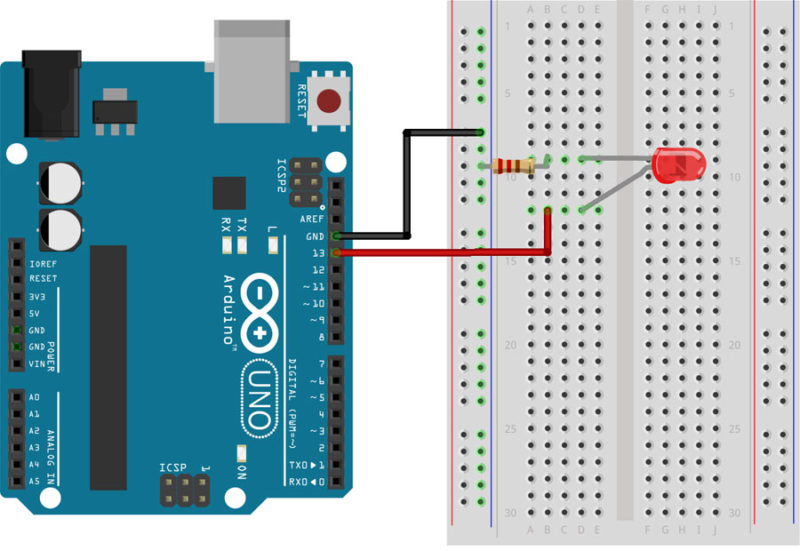
\includegraphics[width=0.5\textwidth, keepaspectratio]{images/ledblink.jpg}
	\caption{Arduino Uno connected to an LED on a breadboard}
	\label{fig:ledblink}
\end{figure}


\subsection{How Hot?}
The objective of this lab is to use a temperature sensor and 5 LEDs controlled by an analog temperature sensor reading. The input level of temperature will light up a different number of LEDs.
\subsubsection{Temperature Sensor Background Knowledge}
\begin{itemize}
    \item It basically measures the degree of hotness or coolness and converts it into a readable unit
    \item A temperature sensor has three terminals: Power (connect to the 3.3V / 5V), Vout (connect to one of the analog inputs), GND (connect to the ground pin). In TinkerCAD, if you hover over the pins, you can see which one is which on the part. 
\end{itemize}
\subsubsection{Reading an analog input}
\begin{enumerate}
  \item Prepare a new circuit canvas and place the following components on to the canvas:
  \item Since this lab requires an \href{https://learn.sparkfun.com/tutorials/analog-vs-digital/}{analog reading}, remember to use the analog-input pins on your Arduino . Likewise, remember to use the \texttt{analogRead()} function when programming your Arduino.
  \item Before you write a program to light up your LEDs, it may be a good idea to use the \texttt{Serial.println()} function. This will create an output on the serial monitor (which can be accessed by clicking the ‘Serial Monitor’ button on the bottom right of your screen) allowing you to create proper divisions for values to light up each LED.
  \item Will your LEDs light up as the temperature sensor readings increase linearly or exponentially? Experiment using different techniques and discuss with your teammates the pros and cons of each method.
  \item Try to make your circuit as compact as possible. Use the least number of wires and try to make sure wires don’t cross each other a lot (this will be a useful trait when creating PCBs)
\end{enumerate}
\subsubsection{Using the \texttt{Serial.println} function and Serial Monitor}
This is a very useful function when experimenting with serial analog inputs, but there is a specific way you need to set it up for this lab. Note that you can use Serial.print() as well, but doing so will have everything printed on one line instead of a new line.
\begin{enumerate}
    \item Inside \texttt{void setup()}, write a function that sets up the data rate in bits per second (baud). It’s okay if you don’t understand what this means right now. Just know that in order to use the serial monitor, you have to establish the data rate for communication. The common rate is 9600 baud. You can set this by writing the function with the following parameter \texttt{Serial.begin(9600)};
    \item Inside \texttt{void loop()}, include \texttt{Serial.println(var)}; directly after your \texttt{analogRead()} function. A good idea might be to have the \texttt{analogRead()} function update a variable and then have the \texttt{Serial.println()} function print the value of the function.
    \item To view your output, you will have to open the Serial Monitor. On the Arduino IDE, you would go to Tools → Serial Monitor. Since we are using TinkerCAD, you will have to open the Code panel and click Serial Monitor on the bottom. Note that you will not see any printed values until you Start Simulation.
\end{enumerate}
    \begin{figure}[ht]
	\center
	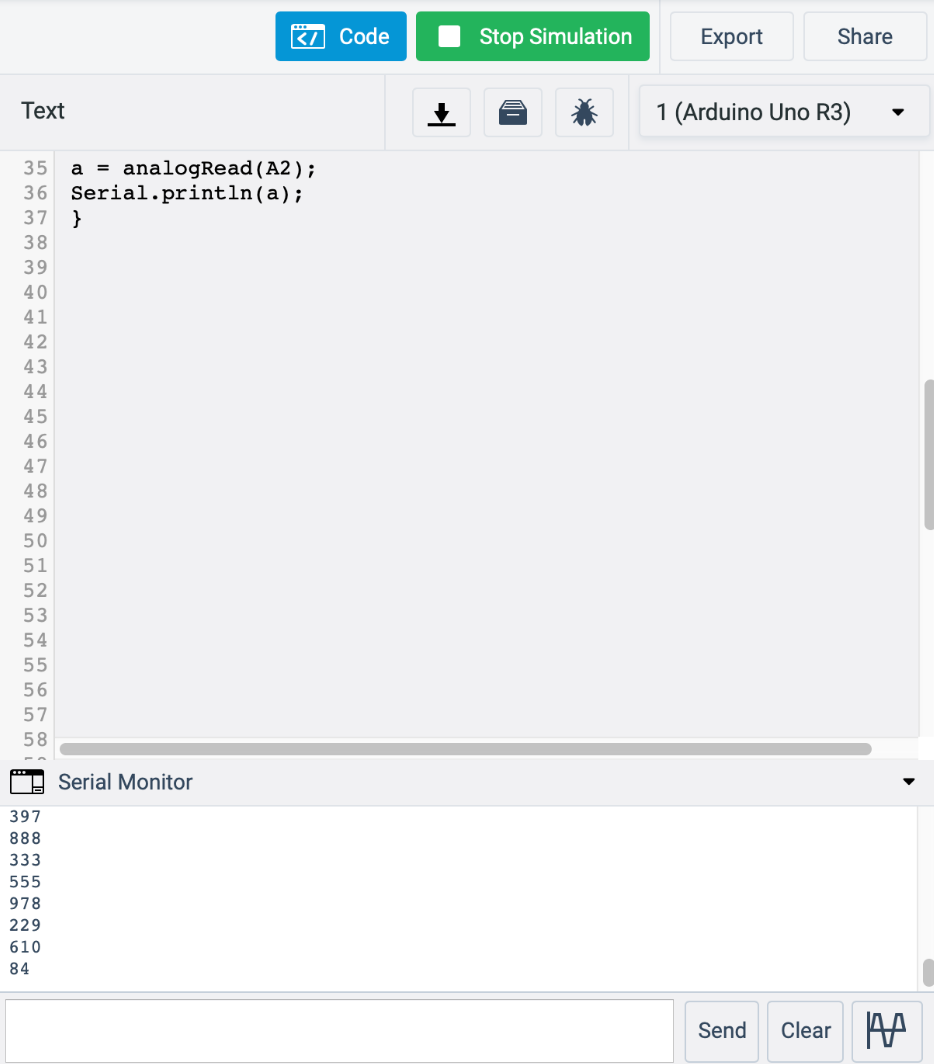
\includegraphics[width=0.5\textwidth, keepaspectratio]{images/serialmonitor.png}
	\caption{Serial Monitor in TinkerCAD}
	\label{fig:serial}
\end{figure}

\section{Materials}
\begin{itemize}
	\item \href{https://www.autodesk.com/education/edu-software/overview}{AutoDesk Education Account}
	\item \href{https://www.tinkercad.com/things/l61Qq635TAR}{TinkerCAD for 2.1}
	\item \href{https://www.tinkercad.com/things/60Ol9dbc90P}{TinkerCAD for 2.2}
\end{itemize}

\section{Relevant Information}
\subsection{TinkerCAD Simulator}
This online CAD works by using drag-and-drop features. You can search for components by using the search bar on the panel to the right. Once you place down a component, you can rotate or delete it using the buttons on the top left of your screen (or click on backspace on your keyboard). To connect components to each other, you can use a breadboard or hover and click from one terminal to another to connect a wire.

If you use a component which requires some code, like an Arduino, you can program the component by clicking the Code button on the top right. After you finish building and programming your circuit, click Start Simulation. You may have an option to view the Serial Monitor/Console. 

Once you succeed with your build, you can share it with team members for review. Alternatively, you can leave comments on other people’s or your own circuit by clicking the Annotation button on the top left. 
\begin{figure}[ht]
	\center
	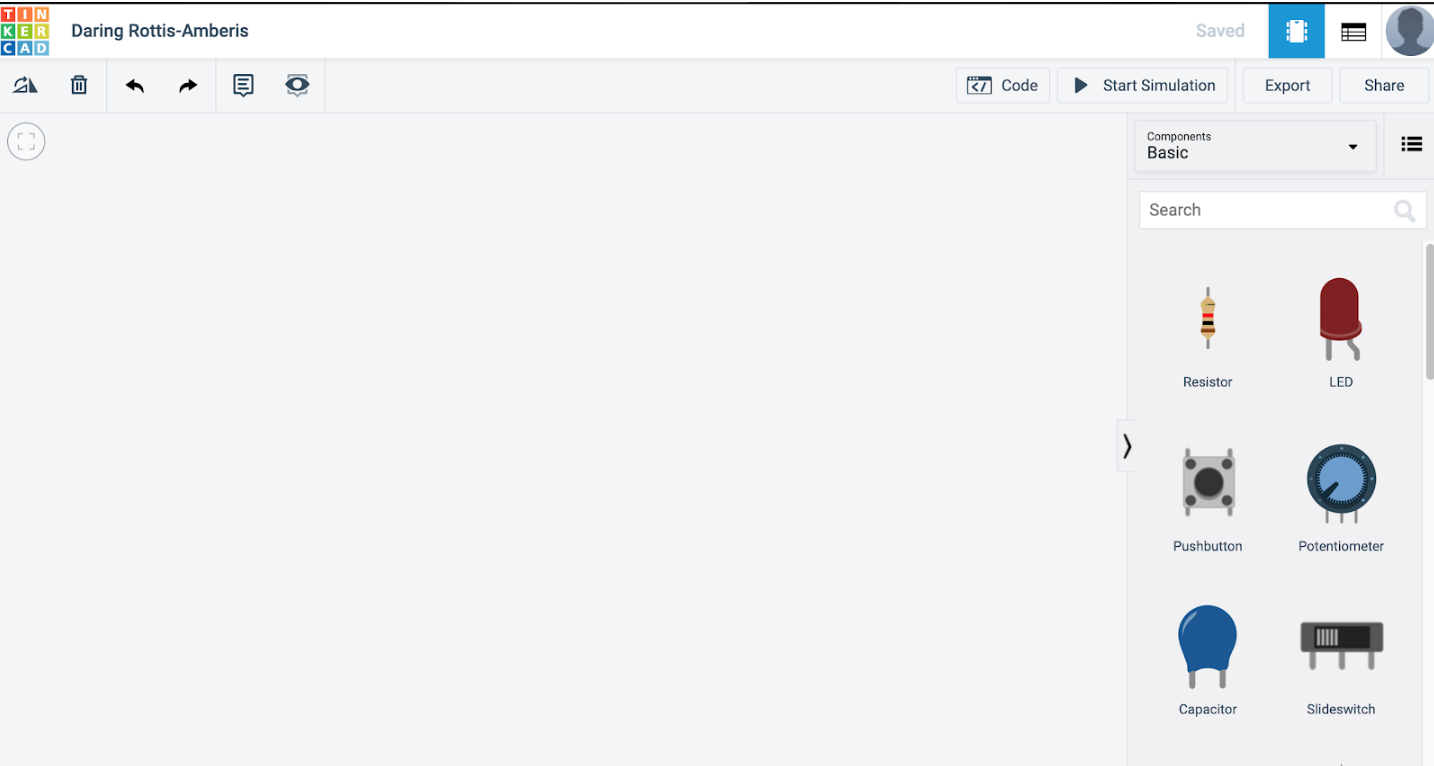
\includegraphics[width=0.8\textwidth, keepaspectratio]{images/tinkercadwindow.png}
	\caption{Creating a new circuit in TinkerCAD}
	\label{fig:window}
\end{figure}

\subsection{Arduino IDE} 
The full official guide for the Arduino can be found \href{https://www.arduino.cc/en/Guide/Environment}{here} \\
\begin{itemize}
    \item The checkmark is the “Verify” button which will compile your code
    \begin{itemize}
        \item Compiling your code means translating your written code from a specific language to a machine executable code
    \end{itemize}
    \item The arrow pointing to the right is the “Upload” button which will compile and load your code on your Arduino
    \item Before you compile make sure to select the port on your computer where your Arduino is connected by going to Tools → Port
\end{itemize}
\begin{figure}[ht]
	\center
	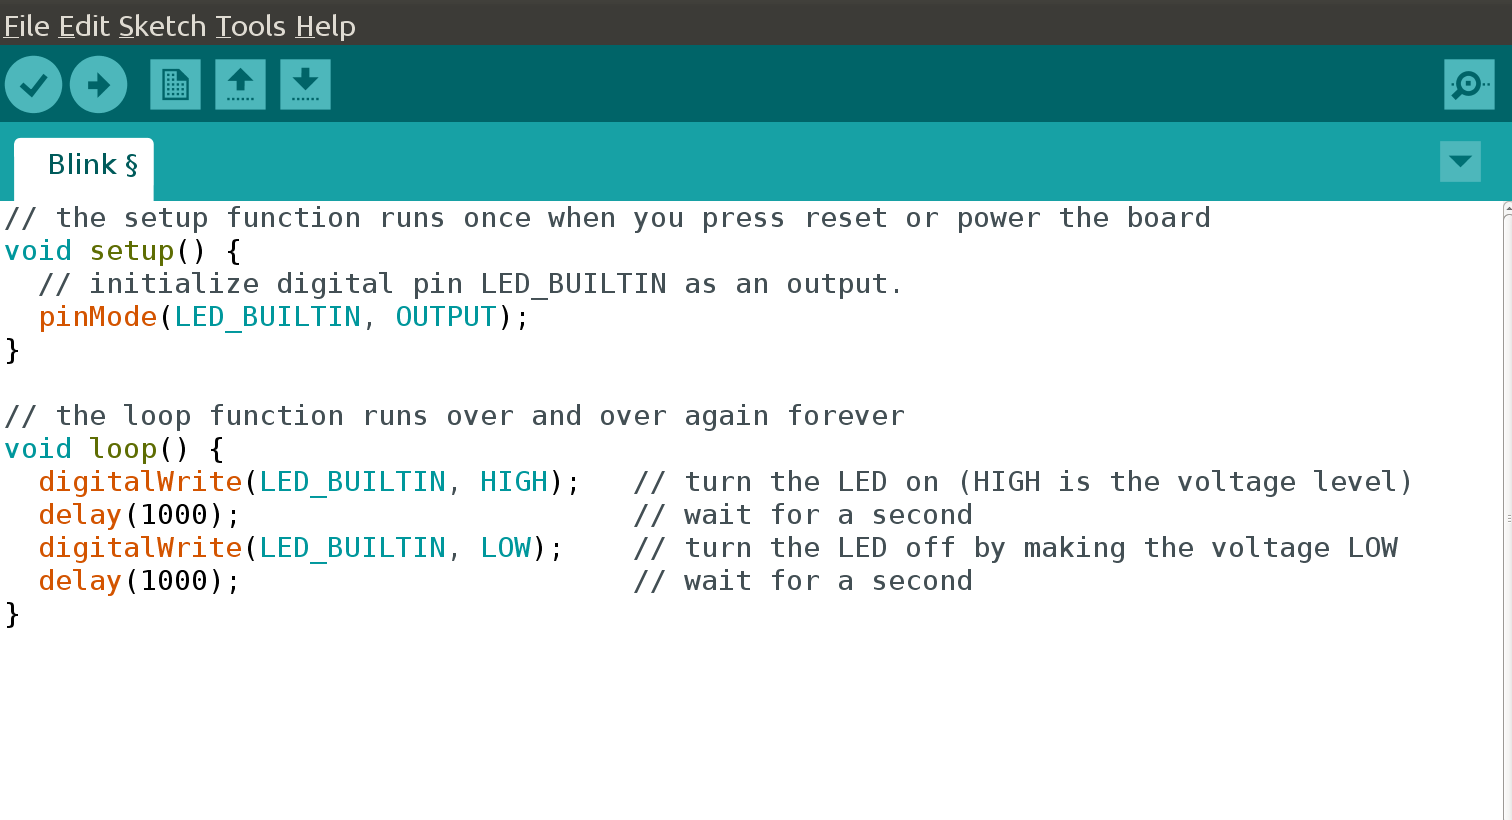
\includegraphics[width=0.9\textwidth, keepaspectratio]{images/arduinoide.png}
	\caption{Arduino IDE with a Blink program}
	\label{fig:arduino}
\end{figure}
The screenshot above is from the Arduino IDE -- the application in which you will write your code and upload the code to your Arduino. The program will blink an on-built LED on the Arduino.

A typical program is split into two parts: the \texttt{setup()} function and the \texttt{loop()} function:
\begin{itemize}
    \item \texttt{setup()} This function is called when the program starts. It’ll run when you power on or reset the Arduino board. Here is where you will initialize variables, set pin modes, etc. 
    \item \texttt{loop()} This function loops consecutively so the code you place here will constantly run
\end{itemize}
Some common functions you should know are outlined below:
\begin{itemize}
    \item \texttt{pinMode(pin, mode)}: Configures the specified pin to behave either as an input or an output
    \begin{itemize}
        \item \texttt{pin} is the number which is located next to the pin on the board
        \item \texttt{mode} determines whether the pin serves as an INPUT or OUTPUT
    \end{itemize}
    \item \texttt{digitalWrite(pin, value)}: Write a high or a low value to a digital pin
    \begin{itemize}
        \item \texttt{pin} references the pin number
        \item \texttt{value} determines whether the output should be given a HIGH or LOW value
    \end{itemize}
    \item \texttt{digitalRead(pin)}: Read a value (high or low) from a specified pin
    \begin{itemize}
        \item \texttt{pin} references the pin number
    \end{itemize}
    \item \texttt{delay(time)}: Pauses the program for a specified amount of time
    \begin{itemize}
        \item \texttt{time} takes a numerical value to represent milliseconds
    \end{itemize}
\end{itemize}
Some more advanced functions include:
\begin{itemize}
    \item \texttt{analogWrite(pin, value)}: Write an analog value to a digital pin with PWM (pulse width modulation)
    \begin{itemize}
        \item \texttt{pin} references the pin number
        \item \texttt{value} determines the output voltage (often based on AREF)
    \end{itemize}
    \item \texttt{analogRead(pin)}: Read an analog value from a specified pin
    \begin{itemize}
        \item \texttt{pin} references the pin number
    \end{itemize}
\end{itemize}


\section{Troubleshooting}
\subsection{Solutions}
We have included the solutions below if you do not complete the lab during the session or if you want to verify your answer. If you need help during the lab ask an instructor!
\begin{itemize}
    \item \href{https://www.tinkercad.com/things/bUqJOIWlYAN}{TinkerCAD Solution for 2.1}
    \item \href{https://www.tinkercad.com/things/1ioFvB93kYq}{TinkerCAD Solution for 2.2}
\end{itemize}




\end{document}